% -----------------------------------------------------------------------------
% Copyright &copy; 2015 Ben Blazak <bblazak@fullerton.edu>  
% This work is licensed under a [Creative Commons Attribution 4.0 International
% License] (http://creativecommons.org/licenses/by/4.0/)  
% -----------------------------------------------------------------------------

% -----------------------------------------------------------------------------
% Copyright &copy; 2015 Ben Blazak <bblazak@fullerton.edu>  
% This work is licensed under a [Creative Commons Attribution 4.0 International
% License] (http://creativecommons.org/licenses/by/4.0/)  
% -----------------------------------------------------------------------------

% - [Which lua environment should I use?] (http://tex.stackexchange.com/a/33102)
\directlua{require('scripts/functions.lua')}

\ifx\question\undefined
  \long\def \question #1{#1}
\fi
\ifx\answer\undefined
  \long\def \answer #1{#1}
\fi

% -----------------------------------------------------------------------------

\def \docTitle  {\directlua{tex.print(doc_title('\jobname'))}}
\def \docAuthor {\question{Name:\hfill{}CWID:\hfill}\answer{Answer Key}}
\def \docClass  {CPSC 121-11}
\def \docSchool {~}
\def \docTerm   {CSUF Fall 2015}

\def \docCopyright {
  \begin{figure}[b!]
    \tiny
    {\answer{\color{red}}\question{\color{.}}\hrule}
    \vspace{2ex}
    \begin{minipage}[c]{0.10\textwidth} \vspace{0ex} \vspace{-1pt}
      
\includegraphics[height=5ex]{images/ccby}
    \end{minipage}
    \begin{minipage}[c]{0.90\textwidth} \vspace{0ex}
      Copyright \copyright{} Ben Blazak \url{bblazak@fullerton.edu}\\
      This work is licensed under a Creative Commons Attribution 4.0
      International License \url{http://creativecommons.org/licenses/by/4.0/}
    \end{minipage}
    \vspace{-.14in}
    \vspace{2ex}
  \end{figure}
}

% -----------------------------------------------------------------------------

\documentclass{article}

\usepackage[includehead,
%             includefoot,
            margin=1in,
            top=.25in,
            headheight=.75in,
            headsep=.25in,
            footskip=.25in,
           ]{geometry}

\usepackage[export]{adjustbox}
\usepackage[fleqn]{amsmath}
\usepackage{amssymb}
\usepackage[shortlabels]{enumitem}
\usepackage{etoolbox}
\usepackage{fancyhdr}
\usepackage{lastpage}
\usepackage[cachedir={.minted-\jobname}]{minted}
\usepackage{tcolorbox}
\usepackage{tikz}
\usepackage[explicit]{titlesec}

\usepackage[T1]{fontenc}
\usepackage[utf8]{inputenc}
\usepackage{lmodern}

\usepackage{xcolor}

% - [Illegal parameter number in definition of \Hy@tempa]
%   (https://kba49.wordpress.com/2013/04/12/illegal-parameter-number-in-definition-of-hytempa/)
\usepackage{hyperref}

% text ------------------------------------------------------------------------

\binoppenalty = 10000  % never break next to a binary operator
\relpenalty   = 10000  % never break next to a relation operator

\setlength{\parindent}{0em}
\setlength{\parskip}{1ex}

\setlist[itemize]{nosep,itemsep=.5ex,parsep=.5ex}

% sections --------------------------------------------------------------------

% - <http://tex.stackexchange.com/a/58299>
\titleformat{name=\section}[block]{\normalfont\Large\bfseries}{}{0em}{#1\ \thesection}
% - <http://tex.stackexchange.com/a/102120>
\titleformat{name=\section,numberless}[block]{\normalfont\Large\bfseries}{}{0em}{#1}

% math ------------------------------------------------------------------------

\setlength{\mathindent}{1cm}

% - "\begin{document}" resets these values, so they have to be treated
%   specially
\AtBeginDocument{
  \setlength{\abovedisplayskip}{1.5ex plus .5ex minus .5ex}
  \setlength{\belowdisplayskip}{1.5ex plus .5ex minus .5ex}
}

% source code -----------------------------------------------------------------

\usemintedstyle{solarizedlight}
\setminted{frame=single}

\fvset{samepage=true}

% header and footer -----------------------------------------------------------

\pagestyle{fancy}

\renewcommand{\headrule}{{\answer{\color{red}}\question{\color{.}}
                          \vskip 0.5ex \hrule height 0.4pt \vskip 0.5ex}}
\renewcommand{\footrule}{{\answer{\color{red}}\question{\color{.}}
                          \vskip 0.5ex \hrule height 0.4pt \vskip 0.5ex}}

\fancyhead[L]{{\answer{\color{red}}\question{\color{.}}\docAuthor}
              {\color{.}\\\docClass}}
\fancyhead[C]{{\color{.}\docSchool\\}}
\fancyhead[R]{{\color{.}\docTerm\\\docTitle}}

\fancyfoot[C]{\thepage{} of \pageref{LastPage}}

% -----------------------------------------------------------------------------
% macros
% -----------------------------------------------------------------------------

% abbreviations ---------------------------------------------------------------

\def \<{\langle}
\def \>{\rangle}

\def \ε{\varepisilon}
\def \θ{\vartheta}
\def \κ{\varkappa}
\def \π{\varpi}
\def \ρ{\varrho}
\def \σ{\varsigma}
\def \φ{\varphi}

\def \Γ{\varGamma}
\def \Δ{\varDelta}
\def \Θ{\varTheta}
\def \Λ{\varLambda}
\def \Ξ{\varXi}
\def \Π{\varPi}
\def \Σ{\varSigma}
\def \Υ{\varUpsilon}
\def \Φ{\varPhi}
\def \Ψ{\varPsi}
\def \Ω{\varOmega}

% special characters ----------------------------------------------------------

\catcode `α = \active \let α \alpha
\catcode `β = \active \let β \beta
\catcode `γ = \active \let γ \gamma
\catcode `δ = \active \let δ \delta
\catcode `ε = \active \let ε \epsilon
\catcode `ζ = \active \let ζ \zeta
\catcode `η = \active \let η \eta
\catcode `θ = \active \let θ \theta
\catcode `ι = \active \let ι \iota
\catcode `κ = \active \let κ \kappa
\catcode `λ = \active \let λ \lambda
\catcode `μ = \active \let μ \mu
\catcode `ν = \active \let ν \nu
\catcode `ξ = \active \let ξ \xi
\catcode `ο = \active \let ο o
\catcode `π = \active \let π \pi
\catcode `ρ = \active \let ρ \rho
\catcode `σ = \active \let σ \sigma
\catcode `τ = \active \let τ \tau
\catcode `υ = \active \let υ \upsilon
\catcode `φ = \active \let φ \phi
\catcode `χ = \active \let χ \chi
\catcode `ψ = \active \let ψ \psi
\catcode `ω = \active \let ω \omega

\catcode `Α = \active \let Α A
\catcode `Β = \active \let Β B
\catcode `Γ = \active \let Γ \Gamma
\catcode `Δ = \active \let Δ \Delta
\catcode `Ε = \active \let Ε E
\catcode `Ζ = \active \let Ζ Z
\catcode `Η = \active \let Η H
\catcode `Θ = \active \let Θ \Theta
\catcode `Ι = \active \let Ι I
\catcode `Κ = \active \let Κ K
\catcode `Λ = \active \let Λ \Lambda
\catcode `Μ = \active \let Μ M
\catcode `Ν = \active \let Ν N
\catcode `Ξ = \active \let Ξ \Xi
\catcode `Ο = \active \let Ο O
\catcode `Π = \active \let Π \Pi
\catcode `Ρ = \active \let Ρ P
\catcode `Σ = \active \let Σ \Sigma
\catcode `Τ = \active \let Τ T
\catcode `Υ = \active \let Υ \Upsilon
\catcode `Φ = \active \let Φ \Phi
\catcode `Χ = \active \let Χ X
\catcode `Ψ = \active \let Ψ \Psi
\catcode `Ω = \active \let Ω \Omega

% other -----------------------------------------------------------------------

\def \docCodeDir {./code/\directlua{tex.print(jobname_root('\jobname'))}/}
\def \docImageDir {./images/\directlua{tex.print(jobname_root('\jobname'))}/}

\long\def \textAnswer #1{\answer{{\color{red!50!black}#1}}}
\long\def \textQuestion #1{\question{{\color{.}#1}}}

\long\def \standardsSection #1{{
  \section*{Standards}
  \def\arraystretch{2}
  \setlength\tabcolsep{1em}
  \begin{tabular}{|r|l|}
    \hline \textbf{Standard} & \textbf{Score} \\\hline #1
  \end{tabular}
  \docCopyright
  \newpage
}
  \def\docCopyright{}
}
\long\def \standards #1{{
  \vspace{-1em}
  \def\arraystretch{2}
  \setlength\tabcolsep{1em}
  \begin{tabular}{|r|l|}
    \hline #1
  \end{tabular}
  \vspace{1em}
}}
\def \standard #1{
  #1 & ~~~ \\\hline
}

\def \evaluateCodeTop #1#2{
  \def\codeFile{\docCodeDir/.#1.cpp.gen.section.#2}
  \IfFileExists{\docCodeDir/.#1.gen.output.gen.section.#2}
               {\def\outputFile{\docCodeDir/.#1.gen.output.gen.section.#2}}
               {\def\outputFile{\docCodeDir/.#1.gen.output.gen.section.all}}
  \par
  \inputminted{cpp}{\codeFile}
  \textQuestion{
    \inputminted[label={\normalsize{}Output},fontsize=\Large]{text}
      {\outputFile.gen.blank}
  }
  \textAnswer{
    \inputminted[label={\normalsize{}Output},fontsize=\Large]{text}
      {\outputFile}
  }
  \par
}
\def \evaluateCodeLeft #1#2{
  \def\codeFile{\docCodeDir/.#1.cpp.gen.section.#2}
  \IfFileExists{\docCodeDir/.#1.gen.output.gen.section.#2}
               {\def\outputFile{\docCodeDir/.#1.gen.output.gen.section.#2}}
               {\def\outputFile{\docCodeDir/.#1.gen.output.gen.section.all}}
  \par
  \begin{minipage}[t]{0.5\linewidth} \vspace{0ex}
    \inputminted{cpp}{\codeFile}
  \end{minipage}
  \begin{minipage}[t]{0.5\linewidth} \vspace{0ex}
    \textQuestion{
      \inputminted[label=Output]{text}{\codeFile.gen.blank}
    }
    \textAnswer{
      \inputminted[label=Output]{text}{\outputFile}
    }
  \end{minipage}
  \par
}

\def \showCodeTop #1#2{
  \def\codeFile{\docCodeDir/.#1.cpp.gen.section.#2}
  \IfFileExists{\docCodeDir/.#1.gen.output.gen.section.#2}
               {\def\outputFile{\docCodeDir/.#1.gen.output.gen.section.#2}}
               {\def\outputFile{\docCodeDir/.#1.gen.output.gen.section.all}}
  \par
  \inputminted{cpp}{\codeFile}
  \vspace{0.5\parskip}
  \inputminted[label=Output]{text}{\outputFile}
  \par
}
\def \showCodeLeft #1#2{
  \def\codeFile{\docCodeDir/.#1.cpp.gen.section.#2}
  \IfFileExists{\docCodeDir/.#1.gen.output.gen.section.#2}
               {\def\outputFile{\docCodeDir/.#1.gen.output.gen.section.#2}}
               {\def\outputFile{\docCodeDir/.#1.gen.output.gen.section.all}}
  \par
  \begin{minipage}[t]{0.5\linewidth} \vspace{0ex}
    \inputminted{cpp}{\codeFile}
  \end{minipage}
  \begin{minipage}[t]{0.5\linewidth} \vspace{0ex}
    \inputminted[label=Output]{text}{\outputFile}
  \end{minipage}
  \par
}



% -----------------------------------------------------------------------------

\begin{document}
\docCopyright

\section*{Standards}
If you are not assessing a standard, please cross out the grade box both here
and on the question page.
\par\vspace{0.4in}
\begin{minipage}[t]{0.33\linewidth}
  \standards{
    \standard{documentation}
    \standard{consistency of style}
  }
\end{minipage}
\begin{minipage}[t]{0.67\linewidth} \vspace{-1.8ex}
  To assess these, write ``+ documentation'' or ``+ consistency of style'' next
  to the grade box for \textit{one} of
  {\color{gray}\{}templates, standard library, exceptions{\color{gray}\}},
  {\color{gray}\{}classes, inheritance, interfaces{\color{gray}\}}, or
  {\color{gray}\{}file I/O{\color{gray}\}}.
  Be sure to demonstrate your mastery of the standard in your answer to the
  question.
\end{minipage}
\par\vspace{0.45in}
\begin{minipage}[t]{1\linewidth}
  \standards{
    \standard{review :: general knowledge}
    \standard{object-oriented programming :: general knowledge}
  }
\end{minipage}
\par\vspace{0.45in}
\begin{minipage}[t]{0.6\linewidth}
  \standards{
    \standard{polymorphism}
    \standard{recursion}
    \standard{pseudocode}
    \standard{searching, sorting, and algorithm analysis}
    \standard{parallel arrays}
    \hline\hline
    \standard{templates}
    \standard{standard library}
    \standard{exceptions}
    \hline\hline
    \standard{debugging and testing correctness}
    \standard{type declarations}
    \standard{pointers and references}
    \standard{memory management and dynamic memory}
  }
\end{minipage}
\begin{minipage}[t]{0.4\linewidth}
  \standards{
    \standard{classes}
    \standard{inheritance}
    \standard{interfaces}
    \hline\hline
    \standard{data types and representation}
    \standard{operators}
    \standard{control flow}
    \standard{arrays}
    \standard{functions}
    \standard{file I/O}
  }
\end{minipage}
\newpage

\newpage

\section{Question}
\standards{
  \standard{review :: general knowledge}
}

Define or describe each of the following:
\textQuestion{\makeDashedLine}
\begin{itemize}
  \item C++ compilation process
    \begin{itemize}
      \item preprocess
        \textAnswer{\par
          \url{http://faculty.cs.niu.edu/~mcmahon/CS241/Notes/compile.html}
        }
        \vfill\textQuestion{\makeDashedLine}
      \item compile
        \textAnswer{\par
          \url{http://faculty.cs.niu.edu/~mcmahon/CS241/Notes/compile.html}
        }
        \vfill\textQuestion{\makeDashedLine}
      \item assemble
        \textAnswer{\par
          \url{http://faculty.cs.niu.edu/~mcmahon/CS241/Notes/compile.html}
        }
        \vfill\textQuestion{\makeDashedLine}
      \item link
        \textAnswer{\par
          \url{http://faculty.cs.niu.edu/~mcmahon/CS241/Notes/compile.html}
        }
        \vfill\textQuestion{\makeDashedLine}
    \end{itemize}
  \item program execution process
    \begin{itemize}
      \item load
        \textAnswer{\par
          \url{https://en.wikipedia.org/wiki/Loader_(computing)}
        }
        \vfill\textQuestion{\makeDashedLine}
      \item run
        \textAnswer{\par
          \url{https://en.wikipedia.org/wiki/Execution_(computing)}
        }
        \vfill\textQuestion{\makeDashedLine}
    \end{itemize}
  \item named constant vs object-like macro
    (e.g.~\mintinline{cpp}{const int ten = 10;} vs
    \mintinline{cpp}{#define TEN 10})
    \textAnswer{\par
      A named constant is like a variable except that its value cannot be
      changed, while an object-like macro is (roughly) a string of code that
      will be replaced by the preprocessor with some other string of code
      before compilation.  This has many implications, depending on how each is
      used, though in many simple cases (with compiler optimization on) the
      generated code is the same.
      \begin{itemize}
        \item \url{http://duramecho.com/ComputerInformation/WhyHowCppConst.html}
        \item \url{https://gcc.gnu.org/onlinedocs/cpp/Object-like-Macros.html}
      \end{itemize}
    }
    \vfill\textQuestion{\makeDashedLine}
  \item bit, byte, word
    \textAnswer{\par
      \begin{itemize}
        \item \url{https://en.wikipedia.org/wiki/Bit}
        \item \url{https://en.wikipedia.org/wiki/Byte}
        \item \url{https://en.wikipedia.org/wiki/Word_(computer_architecture)}
      \end{itemize}
    }
    \vfill
\end{itemize}

\newpage


\newpage

\section{Question}
\standards{
  \standard{object-oriented programming :: general knowledge}
}

Give brief definitions of the following terms:
\textQuestion{\makeDashedLine}
\begin{itemize}
  \item object
    \textAnswer{\par
      A collection of data (what the object is made of) and methods (or member
      functions) on that data (what the object can do, or what messages the
      object understands) having a type (what the object is seen as).
    }
    \vfill\vfill\textQuestion{\makeDashedLine}
  \item class
    \textAnswer{\par
      A description of (or a template (though not in the C++ and Java sense) for
      creating) an object.
    }
    \vfill\textQuestion{\makeDashedLine}
  \item instance
    \textAnswer{\par
      A specific object existing in memory.
    }
    \vfill\textQuestion{\makeDashedLine}
  \item superclass
    \textAnswer{\par
      A class that is a parent of the class to which we are referring (i.e.~a
      class from which we directly or indirectly inherit).
    }
    \vfill\textQuestion{\makeDashedLine}
  \item subclass
    \textAnswer{\par
      A class that is a child of the class to which we are referring (i.e.~a
      class that directly or indirectly inherits from us).
    }
    \vfill\textQuestion{\makeDashedLine}
  \item member
    \textAnswer{\par
      A datum or method belonging to a class.
    }
    \vfill\textQuestion{\makeDashedLine}
  \item method
    \textAnswer{\par
      Or member function.  An action that an object is able to perform, or a
      message that an object is able to understand.
    }
    \vfill\textQuestion{\makeDashedLine}
  \item getters and setters
    \textAnswer{\par
      Methods used for retrieving (getting) or modifying (setting) an object's
      data members.
    }
    \vfill\textQuestion{\makeDashedLine}
  \item accessors and mutators
    \textAnswer{\par
      The same as getters and setters.
    }
    \vfill\textQuestion{\makeDashedLine}
  \item access modifiers
    \begin{itemize}
      \item public
        \textAnswer{\par
          Visible to everyone.
        }
        \vfill\textQuestion{\makeDashedLine}
      \item private
        \textAnswer{\par
          Visible within the class, and to friends.
        }
        \vfill\textQuestion{\makeDashedLine}
      \item protected
        \textAnswer{\par
          Visible within the class, to child classes, and to friends.
        }
        \vfill
        \vfill
    \end{itemize}
\end{itemize}

\newpage



\newEvenPage

\section{Question}
\standards{
  \standard{polymorphism}
}

Show the output of the following program:
\evaluateCodeTop{polymorphism-1}{all}
\vspace{3ex}

What (if anything) is wrong with the code that is commented out above?
\textAnswer{\par
  It is possible to have a pointer of type superclass pointing to an object of
  type subclass, but not the other way around.  This makes sense because a
  child class will always have the same members as its parent (though, not
  always with the same access specifiers), but the reverse is rarely true.
  Also, conceptually, a \mintinline{cpp}{SmallDog} is always a
  \mintinline{cpp}{Dog}, so we may treat it as one; but a \mintinline{cpp}{Dog}
  will not always be a \mintinline{cpp}{SmallDog}, and it would be a mistake to
  assume we could treat all \mintinline{cpp}{Dog}s as
  \mintinline{cpp}{SmallDog}s.
}

\newpage


\newpage

\section{Question}
\standards{
  \standard{recursion}
}

Write a recursive function called \mintinline{cpp}{sum_from_1_to} that takes as
an argument some positive integer \mintinline{cpp}{n} and returns the sum of
all the integers between \mintinline{cpp}{1} and \mintinline{cpp}{n},
inclusive.  If the value passed is invalid, the function should return
\mintinline{cpp}{0}.  For example:

\showCodeLeft{recursion-1}{main}

\textAnswer{\inputminted{cpp}{\docCodeDir/.recursion-1.cpp.gen.section.function}}

\newpage


\newpage

\section{Question}
\standards{
  \standard{pseudocode}
  \standard{searching, sorting, and algorithm analysis}
}

Do \textbf{one} of the following:
\begin{itemize}
  \item Write pseudocode for the merge sort algorithm.
  \item Write pseudocode for the selection sort algorithm.
\end{itemize}

\textAnswer{{\par
  \subsection*{merge sort}
  \begin{itemize}
    \item If the list received is less than 2 elements long then return it
      unchanged.
    \item Otherwise, do the following:
      \begin{itemize}
        \item Split the list in half (putting the odd element, if any, in
          either half).
        \item Recursively merge sort the left half.
        \item Recursively merge sort the right half.
        \item Merge the sorted left and right halves together as follows:
          \begin{itemize}
            \item Create a new empty list named \mintinline{cpp}{sorted}.
            \item While both lists are nonempty:
              \begin{itemize}
                \item Compare the first element of each list.
                \item Take the smaller element out of the list it is in, and
                  put it in \mintinline{cpp}{sorted}.
              \end{itemize}
            \item Take the remaining elements from the nonempty list, and place
              them in order at the end of \mintinline{cpp}{sorted}.
            \item Return \mintinline{cpp}{sorted}.
          \end{itemize}
      \end{itemize}
  \end{itemize}

  \subsection*{selection sort}
  \begin{itemize}
    \item For each element in the list, in order from left to right:
      \begin{itemize}
        \item Find the minimum element between that element and the end of the
          list (inclusive)
        \item If that element is not the minimum element, swap it with the
          minimum element.
      \end{itemize}
  \end{itemize}
}}

\textQuestion{\makePageQuadrilleRuled}

\newpage


\newpage

\section{Question}
\standards{
  \standard{parallel arrays}
}

When for some reason \mintinline{cpp}{class}es or \mintinline{cpp}{struct}s are
undesirable for holding associated data, one might use parallel arrays.  For
example, instead of having an array of \mintinline{cpp}{struct} instances for
some \mintinline{cpp}{struct} that contains two fields, one might have two
arrays, where the first array contains the values that would have been in the
first field and the second array contains the corresponding values that would
have been in the second field.

Write a \mintinline{cpp}{main()} that does the same thing as the one below,
except using parallel arrays.  That is, instead of using an array of
\mintinline{cpp}{Person} instances, use two arrays: one for the names, and one
for the ages.

\inputminted{cpp}{\docCodeDir/.parallel-1.cpp.gen.section.all}

\textAnswer{\inputminted{cpp}{\docCodeDir/.parallel-1.cpp.gen.section.arrays}}

\newpage



\newEvenPage

\section{Question}
\standards{
  \standard{templates}
}

Leave a bit of room at the top of the page for comments,
\mintinline{cpp}{#include} directives, and \mintinline{cpp}{using} statements.

Write a function template named \mintinline{cpp}{add} capable of taking two
arguments of any type (so long as they are both of the same type) and returning
their sum (using the \mintinline{cpp}{+} operator).

Write a class template named \mintinline{cpp}{Complex} that accepts one
template argument, \mintinline{cpp}{T}, and has two public data members of type
\mintinline{cpp}{T}: \mintinline{cpp}{r} to store the real part, and
\mintinline{cpp}{i} to store the imaginary part.  Overload the
\mintinline{cpp}{+} operator so that two \mintinline{cpp}{Complex<T>} objects
may be added (prototype this method in the class definition, and define it
directly below).  Recall that the formula for adding two complex numbers
$(a+bi)$ and $(c+di)$ is
\begin{align*}
  (a+bi)+(c+di) &= (a+c) + (b+d)i
\end{align*}

Write a \mintinline{cpp}{main()} to do the following:
\begin{itemize}
  \item Create two objects, \mintinline{cpp}{a} and \mintinline{cpp}{b}, using
    the class template \mintinline{cpp}{Complex} with the template argument
    \mintinline{cpp}{int}.
  \item For \mintinline{cpp}{a}, set the real part to \mintinline{cpp}{1} and
    the imaginary part to \mintinline{cpp}{2}.
  \item For \mintinline{cpp}{b}, set the real part to \mintinline{cpp}{3} and
    the imaginary part to \mintinline{cpp}{4}.
  \item Create an object named \mintinline{cpp}{c} of the same type as
    \mintinline{cpp}{a} and \mintinline{cpp}{b}, and use the
    \mintinline{cpp}{add} function template to set it equal to the sum of
    \mintinline{cpp}{a} and \mintinline{cpp}{b}.
  \item Output the value of \mintinline{cpp}{c} using the following statement:
    \mintinline{cpp}{cout << c.r << " + " << c.i << "i\n";}.
\end{itemize}

\newOddPage
\textQuestion{\makePageQuadrilleRuled}
\textAnswer{\inputminted{cpp}{\docCodeDir/.templates-2.cpp.gen.section.all}}

\newOddPage
\textQuestion{\makePageQuadrilleRuled}
\textAnswer{~}

\newpage


\newEvenPage

\section{Question}
\standards{
  \standard{standard library}
}

Leave a bit of room at the top of the page for comments,
\mintinline{cpp}{#include} directives, and \mintinline{cpp}{using} statements.

Overload the stream insertion operator for objects of type
\mintinline{cpp}{vector<int>} (or optionally, use templates to overload it for
\mintinline{cpp}{vector}s of any type).  The output for a vector containing the
integers \mintinline{cpp}{1}, \mintinline{cpp}{2}, and \mintinline{cpp}{3} (for
example) should be \mintinline{text}{( 1 2 3 )}.

Write a \mintinline{cpp}{main()} to do the following:
\begin{itemize}
  \item Create and initialize (in the same statement) an object named
    \mintinline{cpp}{v} of type \mintinline{cpp}{vector<int>} holding the
    values \mintinline{cpp}{1}, \mintinline{cpp}{2}, and \mintinline{cpp}{3}
    (in that order).
  \item Use the method on \mintinline{cpp}{vector<int>} that adds an element to
    the end of the vector (or pushes an element onto the back of the vector) to
    add \mintinline{cpp}{4} to the end of \mintinline{cpp}{v}.
  \item Use the \mintinline{cpp}{[]} operator to change the element at index
    \mintinline{cpp}{1} to \mintinline{cpp}{5}.
  \item Use the overloaded stream insertion operator to print
    \mintinline{cpp}{v} to standard output, \textbf{and indicate the output}.
\end{itemize}

\newOddPage
\textQuestion{\makePageQuadrilleRuled}
\textAnswer{\showCodeTop{standard-2}{all}}

\newpage


\newEvenPage

\section{Question}
\standards{
  \standard{exceptions}
}

Leave a bit of room at the top of the page for comments,
\mintinline{cpp}{#include} directives, and \mintinline{cpp}{using} statements.

Write a \mintinline{cpp}{class} named \mintinline{cpp}{MyException} that
inherits from \mintinline{cpp}{std::exception}.  Overload the
\mintinline{cpp}{what()} method to return \mintinline{cpp}{"This is the error
message for MyException"}.

Write a \mintinline{cpp}{class} named \mintinline{cpp}{MyClass} that has a
public constructor that does nothing but throw a \mintinline{cpp}{MyException}.

Write a \mintinline{cpp}{main()} to do the following:
\begin{itemize}
  \item Try to create an instance of \mintinline{cpp}{MyClass}.  If this
    succeeds, the program should output \mintinline{cpp}{"It worked!\n"}.
  \item Catch exceptions of type \mintinline{cpp}{MyException} by reference.
    If one is caught, the program should output
    \mintinline{cpp}{"It didn't work.  The error message was:\n"}, followed by
    the error message returned by the \mintinline{cpp}{what()} method of the
    exception that was caught, followed by a newline.
\end{itemize}

Indicate the output this program will produce.

\newOddPage
\textQuestion{\makePageQuadrilleRuled}
\textAnswer{\showCodeTop{exceptions-1}{all}}

\newpage



\newpage

% mostly from reassessment-09

\section{Question}
\standards{
  \standard{debugging and testing correctness}
}

\vspace{3.5ex}

Correct each of the following code sections.

\vspace{3.5ex}
\begin{itemize}
  \item \correctCodeTop{debugging-1}{max} \vspace{7ex}
  \item \correctCodeTop{debugging-1}{void} \vspace{7ex}
    \newpage
  \item \correctCodeTop{debugging-1}{equals} \vspace{7ex}
  \item \correctCodeTop{debugging-1}{or} \vspace{7ex}
    \newpage
  \item \correctCodeTop{debugging-1}{for} \vspace{7ex}
  \item \correctCodeTop{debugging-1}{infinite} \vspace{7ex}
  \item \correctCodeTop{debugging-1}{uninitialized} \vspace{7ex}
\end{itemize}

\newpage


\newpage

% from reassessment-16

\section{Question}
\standards{
  \standard{type declarations}
}

\section*{Instructions}

{
  \long\def\answer#1{#1}
  Write declarations for the following descriptions, and descriptions for the
  following declarations:
  \begin{itemize}
    \item \mintinline{cpp}{int i}
      \textAnswer{\par{}declare i as int}
    \item declare a as array 3 of int
      \textAnswer{\par{}\mintinline{cpp}{int a[3]}}
  \end{itemize}
}

\section*{Questions}

Write declarations for the following descriptions, and descriptions for the
following declarations:
\begin{itemize}

  \item declare p as pointer to int
    \textAnswer{\par{}\mintinline{cpp}{int * p}}
    \vfill

  \item declare r as reference to int
    \textAnswer{\par{}\mintinline{cpp}{int & r}}
    \vfill

  \item \mintinline{cpp}{int (*p)[3]}
    \textAnswer{\par{}declare p as pointer to array 3 of int}
    \vfill

  \item \mintinline{cpp}{int (&r)[3]}
    \textAnswer{\par{}declare r as reference to array 3 of int}
    \vfill

  \item \mintinline{cpp}{void (*p)()}
    \textAnswer{\par{}declare p as pointer to function returning void}
    \vfill

  \item declare p as pointer to function (int, array of int) returning int
    \textAnswer{\par{}\mintinline{cpp}{int (*p)(int, int[])}}
    \vfill

\end{itemize}

\newpage


\newpage

% mostly from reassessment-15

\section{Question}
\standards{
  \standard{pointers and references}
}

\begin{itemize}

  \item Write statements to do the following:
    \begin{itemize}
      \item Declare an \mintinline{cpp}{int} named \mintinline{cpp}{i} and set
        it equal to \mintinline{cpp}{3}.
      \item Declare a pointer named \mintinline{cpp}{p} and use it to set
        \mintinline{cpp}{i} equal to \mintinline{cpp}{4}.
      \item Declare a reference named \mintinline{cpp}{r} and use it to set
        \mintinline{cpp}{i} equal to \mintinline{cpp}{5}.
      \item Output the value of \mintinline{cpp}{i}, the value pointed to by
        \mintinline{cpp}{p}, and the value referenced by \mintinline{cpp}{r},
        separated by whitespace, and \textbf{indicate the results of this
        statement}.
    \end{itemize}
    \textAnswer{\showCodeLeft{pointers-1-1}{all}}
    \vfill

  \item Show the output of the following program:
    \evaluateCodeLeft{pointers-1-2}{all}

    \filbreak

  \item Show the output of the following program.  Recall that
    \mintinline{cpp}{uintptr_t} is an unsigned integer type capable of
    storing any valid pointer value without loss of precision, and that
    \mintinline{cpp}{(uintptr_t)a} is a C style cast of \mintinline{cpp}{a} to
    type \mintinline{cpp}{uintptr_t}.
    \evaluateCodeTop{pointers-1-3}{all}
    \vspace{3ex}

  \item List one similarity between an array and a pointer to the array's first
    element.
    \textAnswer{\par
      \begin{itemize}
        \item Either may be used to access any element of the array, with the
          same syntax.
        \item They both convert to the same integral value.
        \item $\cdots$
      \end{itemize}
    }
    \vfill

  \item List one difference between an array and a pointer to the array's first
    element.
    \textAnswer{\par
      \begin{itemize}
        \item They have different type.
        \item The pointer may be assigned to, whereas the array may not.
        \item Taking \mintinline{cpp}{sizeof(p)} and
          \mintinline{cpp}{sizeof(a)} (assuming the array is called
          \mintinline{cpp}{a} and the pointer is called \mintinline{cpp}{p})
          will give different results.
        \item $\cdots$
      \end{itemize}
    }
    \vfill

\end{itemize}

\newpage


\newpage

% from reassessment-10

\section{Question}
\standards{
  \standard{memory management and dynamic memory}
}

\begin{itemize}

  \item Given a \mintinline{cpp}{const int SIZE} set to some positive value,
    use either the C style functions or the C++ style operators to write
    statements to do the following:
    \begin{itemize}
      \item Dynamically allocate memory for an array of \mintinline{cpp}{SIZE}
        \mintinline{cpp}{double}s, and store the resulting pointer to the first
        element in a variable of the appropriate type.
      \item Deallocate the dynamically allocated memory.
    \end{itemize}
    \textAnswer{\inputminted{cpp}{\docCodeDir/.memory-1.cpp.gen.section.all}}
    \vfill

  \item In what section of memory are automatic variables placed?
    \textAnswer{\par
      the stack
    }
    \vfill

  \item In what section of memory are dynamically allocated variables placed?
    \textAnswer{\par
      the heap (when using C style functions) or the free store (when using C++
      style operators) (though the free store is often informally referred to
      as the heap)
    }
    \vfill

  \item What happens when you dynamically allocate memory, but fail to
    deallocate it?
    \textAnswer{\par
      The memory remains allocated to your program until the program is
      terminated (at which time \textit{all} memory in use by your program is
      reclaimed by the operating system).  This is known as a memory leak.
    }
    \vfill

  \item What happens when you deallocate a block of dynamically allocated
    memory, but keep a pointer to the beginning of the block?
    \textAnswer{\par
      The pointer may still be used in some ways, but dereferencing it leads to
      undefined behavior.  This is known as a dangling pointer.
    }
    \vfill

\end{itemize}

\newpage


% 
\newEvenPage

% code from reassessment-19

\standards{
  \standard{classes}
  \standard{inheritance}
}

Leave a bit of room at the top of the page for comments,
\mintinline{cpp}{#include} directives, and \mintinline{cpp}{using} statements.

Write a class named \mintinline{cpp}{Rectangle} that has two private data
members of type \mintinline{cpp}{double}: \mintinline{cpp}{length}, and
\mintinline{cpp}{width}.  Write a constructor capable of initializing both
private data members.  Write a method named \mintinline{cpp}{area} that returns
the product of \mintinline{cpp}{length} and \mintinline{cpp}{witdh} as a
\mintinline{cpp}{double}.

Write a class named \mintinline{cpp}{Square} that inherits from
\mintinline{cpp}{Rectangle} and has no non-inherited data members.  Write a
constructor that takes a single argument named \mintinline{cpp}{edge}, and
passes this argument (for both parameters) to the parent constructor (in the
initialization list).

Write a \mintinline{cpp}{main()} to do the following:
\begin{itemize}
  \item Create a \mintinline{cpp}{Rectangle} named \mintinline{cpp}{r} and a
    \mintinline{cpp}{Square} named \mintinline{cpp}{s}, initialize them both,
    and use the \mintinline{cpp}{area} method on each as appropriate, to
    produce the following output:
    \inputminted[label=Output]{text}{\docCodeDir/.classes,inheritance-1.gen.output.gen.section.all}
\end{itemize}

\newOddPage
\textQuestion{\makePageQuadrilleRuled}
\textAnswer{\inputminted{cpp}{\docCodeDir/.classes,inheritance-1.cpp.gen.section.all}}

\newpage


\newEvenPage

% code from reassessment-11

\section{Question}
\standards{
  \standard{interfaces}
}

Recall that an interface is an abstract class, and an abstract class is a class
with at least one pure virtual method.

Leave a bit of room at the top of the page for comments,
\mintinline{cpp}{#include} directives, and \mintinline{cpp}{using} statements.

Write an interface named \mintinline{cpp}{Automobile} that has two private data
members of type \mintinline{cpp}{double}: \mintinline{cpp}{fuel}, and
\mintinline{cpp}{speed}.  Remember to declare and define a virtual destructor
(all interface classes should have a virtual destructor).  Declare and define
(inline) virtual getters and setters for both private data members.  Declare
the following pure virtual methods, all of which take no arguments and return
void: \mintinline{cpp}{turnLeft}, \mintinline{cpp}{turnRight},
\mintinline{cpp}{raiseHydraulics}, \mintinline{cpp}{spinRims}.

\newOddPage
\textQuestion{\makePageQuadrilleRuled}
\textAnswer{\inputminted{cpp}{\docCodeDir/.interfaces-1.cpp.gen.section.all}}

\newpage


% 
\newpage

% mostly from reassessment-08

\section{Question}
\standards{
  \standard{data types and representation}
}

\begin{itemize}

  \item Complete the following table for a typical 64 bit system:

    {
      \def\arraystretch{2}
      \begin{tabular}{|c|c|c|}
        \hline
        \textbf{Literal}
        & \textbf{\hbox to 2in{\hfill{}Type\hfill}}
        & \textbf{Size (in bytes)}
        \\\hline
        \mintinline{cpp}{true}
        & \textAnswer{\mintinline{cpp}{bool}}
        & \textAnswer{1}
        \\\hline
        \mintinline{cpp}{3}
        & \textAnswer{\mintinline{cpp}{int}}
        & \textAnswer{4}
        \\\hline
        \mintinline{cpp}{'a'}
        & \textAnswer{\mintinline{cpp}{char}}
        & \textAnswer{1}
        \\\hline
        \mintinline{cpp}{3.14}
        & \textAnswer{\mintinline{cpp}{double}}
        & \textAnswer{8}
        \\\hline
        \mintinline{cpp}{3.14F}
        & \textAnswer{\mintinline{cpp}{float}}
        & \textAnswer{4}
        \\\hline
        \mintinline{cpp}{"hello world"}
        & \textAnswer{\mintinline{cpp}{const char[12]}}
        & \textAnswer{12}
        \\\hline
      \end{tabular}
    }
    \vspace{3ex}

  \item Complete the following table:

    {
      \def\arraystretch{2}
      \begin{tabular}{|c|c|c|}
        \hline
        \textbf{binary}
        & \textbf{decimal}
        & \textbf{hexadecimal}
        \\\hline
        \mintinline{cpp}{0b0111}
        & \textAnswer{\mintinline{cpp}{7}}
        & \textAnswer{\mintinline{cpp}{0x7}}
        \\\hline
        \textAnswer{\mintinline{cpp}{0b1011}}
        & \mintinline{cpp}{11}
        & \textAnswer{\mintinline{cpp}{0xB}}
        \\\hline
        \textAnswer{\mintinline{cpp}{0b1101}}
        & \textAnswer{\mintinline{cpp}{13}}
        & \mintinline{cpp}{0xD}
        \\\hline
      \end{tabular}
    }
    \vspace{3ex}

  \item What would be the minimum and maximum values of a signed 3-bit integer?
    \textAnswer{\par
      $-2^{3-1} = -4$ and $2^{3-1}-1 = 3$
    }
    \vfill

  \item What would be the minimum and maximum values of a unsigned 3-bit
    integer?
    \textAnswer{\par
      $0$ and $2^3-1 = 7$
    }
    \vfill

\end{itemize}

\newpage


\newpage

\section{Question}
\standards{
  \standard{operators}
}

\begin{itemize}

  \item Show the output of the following program:
    \evaluateCodeLeft{operators-1}{all}
    \vspace{3ex}

  \item Evaluate the following statement piece by piece, using the method shown
    in class (if you are unsure of how this should look, please ask).  If any
    portion of this statement would produce a runtime error (e.g.~by dividing
    by \mintinline{cpp}{0}) stop evaluating at that point, and explain.

    \vspace{2ex}
    \mintinline[fontsize=\Large]{cpp}{1 + 1 - 1 / 1 * + 1 - - - 1 && 1 == ! 1 || 1 + 1 >= 1 / 1 % 1}
    \textAnswer{\par
      \vspace{-1.9em}
      \hspace{-1.2ex}
      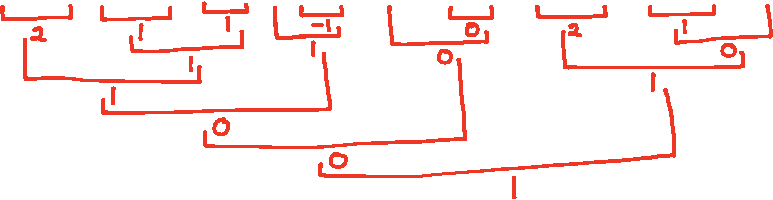
\includegraphics[width=6.37in]{\docImageDir/operators-1}
    }
    \vfill

\end{itemize}

\newpage


\newpage

\section{Question}
\standards{
  \standard{control flow}
}

Use two \mintinline{cpp}{for} loops (one inside the other, and without any
conditionals) to produce the following output:

\inputminted[label=Output]{text}{\docCodeDir/.control-1.gen.output.gen.section.all}
\textAnswer{\inputminted{cpp}{\docCodeDir/.control-1.cpp.gen.section.all}}

\newpage


\newpage

% from reassessment-14

\def\memoryImage{%
  \par\medskip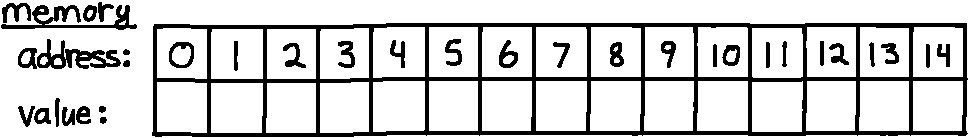
\includegraphics[width=\linewidth,valign=t]{\docImageDir/memory}%
}

\section{Question}
\standards{
  \standard{arrays}
}

\section*{Instructions}

For questions with a picture illustrating memory, assume that the memory slots
are one \mintinline{cpp}{int} wide, and use ``?'' in a slot to indicate that it
contains an undefined value.  For each array, label an appropriately sized
group of slots with the array name, and fill in the slots with the array's
values.

\vspace{2.7ex}
\begin{minipage}[t]{0.5\linewidth} \vspace{0ex}
  \vspace{-2.7ex}
  \memoryImage
  \par
  \vspace{-0.63in}
  \hspace{0.45in}
  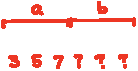
\includegraphics[width=1.15in]{\docImageDir/arrays-example}
\end{minipage}
\begin{minipage}[t]{0.5\linewidth} \vspace{0ex}
  \inputminted{cpp}{\docCodeDir/.arrays-example.cpp.gen.section.array}
\end{minipage}

\section*{Questions}

\begin{itemize}

  \item What is the index of the first element of an array?
    \textAnswer{\par
      Answer: \mintinline{cpp}{0}
    }
    \vfill

  \item What is the index of the last element of any array that holds 7 values?
    \textAnswer{\par
      Answer: \mintinline{cpp}{6}
    }
    \vfill

  \item What happens when you access an element of the array that does not
    exist?
    \textAnswer{\par
      If the program is allowed to access the location in memory then that
      location in memory is accessed as if it were an element of the array
      (regardless of what's actually there).  If the program doesn't have
      access to the location in memory, a segmentation fault (segfault) will
      occur, and the operating system will kill the process.
    }
    \vfill
    \vfill

  \item \memoryImage
    \textAnswer{\par
      \par
      \vspace{-1.12in}
      \hspace{0.9in}
      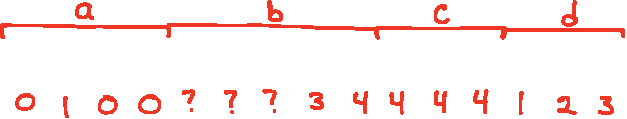
\includegraphics[width=5.2in]{\docImageDir/arrays-1}
    }
    \inputminted{cpp}{\docCodeDir/.arrays-1.cpp.gen.section.array}

\end{itemize}

\newpage


\newpage

\section{Question}
\standards{
  \standard{functions}
}

Assuming that all necessary headers have been included and all required symbols
are in the standard namespace, do the following:

\begin{itemize}

  \item Write a prototype and definition for a function named
    \mintinline{cpp}{abs} that accepts one \mintinline{cpp}{int} and returns
    the absolute value as an \mintinline{cpp}{int}.
    \textAnswer{\showCodeLeft{functions-1}{abs}}
    \vfill

  \item Write a prototype and definition for a function named
    \mintinline{cpp}{swap} that accepts two \mintinline{cpp}{int}s, both passed
    by reference, and swaps their values.
    \textAnswer{\showCodeLeft{functions-1}{swap}}
    \vfill

  \item Write a \mintinline{cpp}{main()} to do the following:
    \begin{itemize}
      \item Let \mintinline{cpp}{int a = 5, b = -7;}.
      \item Output the value returned by \mintinline{cpp}{abs} when called with
        \mintinline{cpp}{a} as its argument, and the value returned by
        \mintinline{cpp}{abs} when called with \mintinline{cpp}{b} as its
        argument, separated by whitespace, followed by a newline.
      \item Output the values of \mintinline{cpp}{a} and \mintinline{cpp}{b},
        separated by whitespace, followed by a newline.
      \item Call \mintinline{cpp}{swap} with \mintinline{cpp}{a} and
        \mintinline{cpp}{b} as its arguments.
      \item Output the values of \mintinline{cpp}{a} and \mintinline{cpp}{b},
        separated by whitespace, followed by a newline.
    \end{itemize}
  \item Indicate the output of \mintinline{cpp}{main()}.
    \textAnswer{\showCodeLeft{functions-1}{main}}
    \vfill

\end{itemize}

\newpage


\newEvenPage

\section{Question}
\standards{
  \standard{file I/O}
}

Given

\inputminted[label={file-io-input.txt}]{text}{\docCodeDir/file-io-input.txt}

write an entire program (including \mintinline{cpp}{#include} directives and
\mintinline{cpp}{using} statements) to generate

\inputminted[label={file-io-output.gen.txt}]{text}{\docCodeDir/file-io-output.gen.txt}

without hard coding the number of integers to read in.  Be sure to check that
opening each file succeeded before reading from or writing to it, and
\mintinline{cpp}{return 1} from \mintinline{cpp}{main()} if it did not.

\newOddPage
\textQuestion{\makePageQuadrilleRuled}
\textAnswer{\inputminted{cpp}{\docCodeDir/.file-io.cpp.gen.section.all}}

\newpage



\end{document}

